Recall from Chapter 4 that explicit ND-range and hierarchical parallel kernels organize work-items into work-groups and that the work-items in a workgroup are guaranteed to execute concurrently. This property is important, because when work-items are guaranteed to execute concurrently, the workitems in a work-group can cooperate to solve a problem.\par

\hspace*{\fill} \par %插入空行
Figure 9-1. Two-dimensional ND-range of size (8, 8) divided into four work-groups of size (4,4)
\begin{center}
	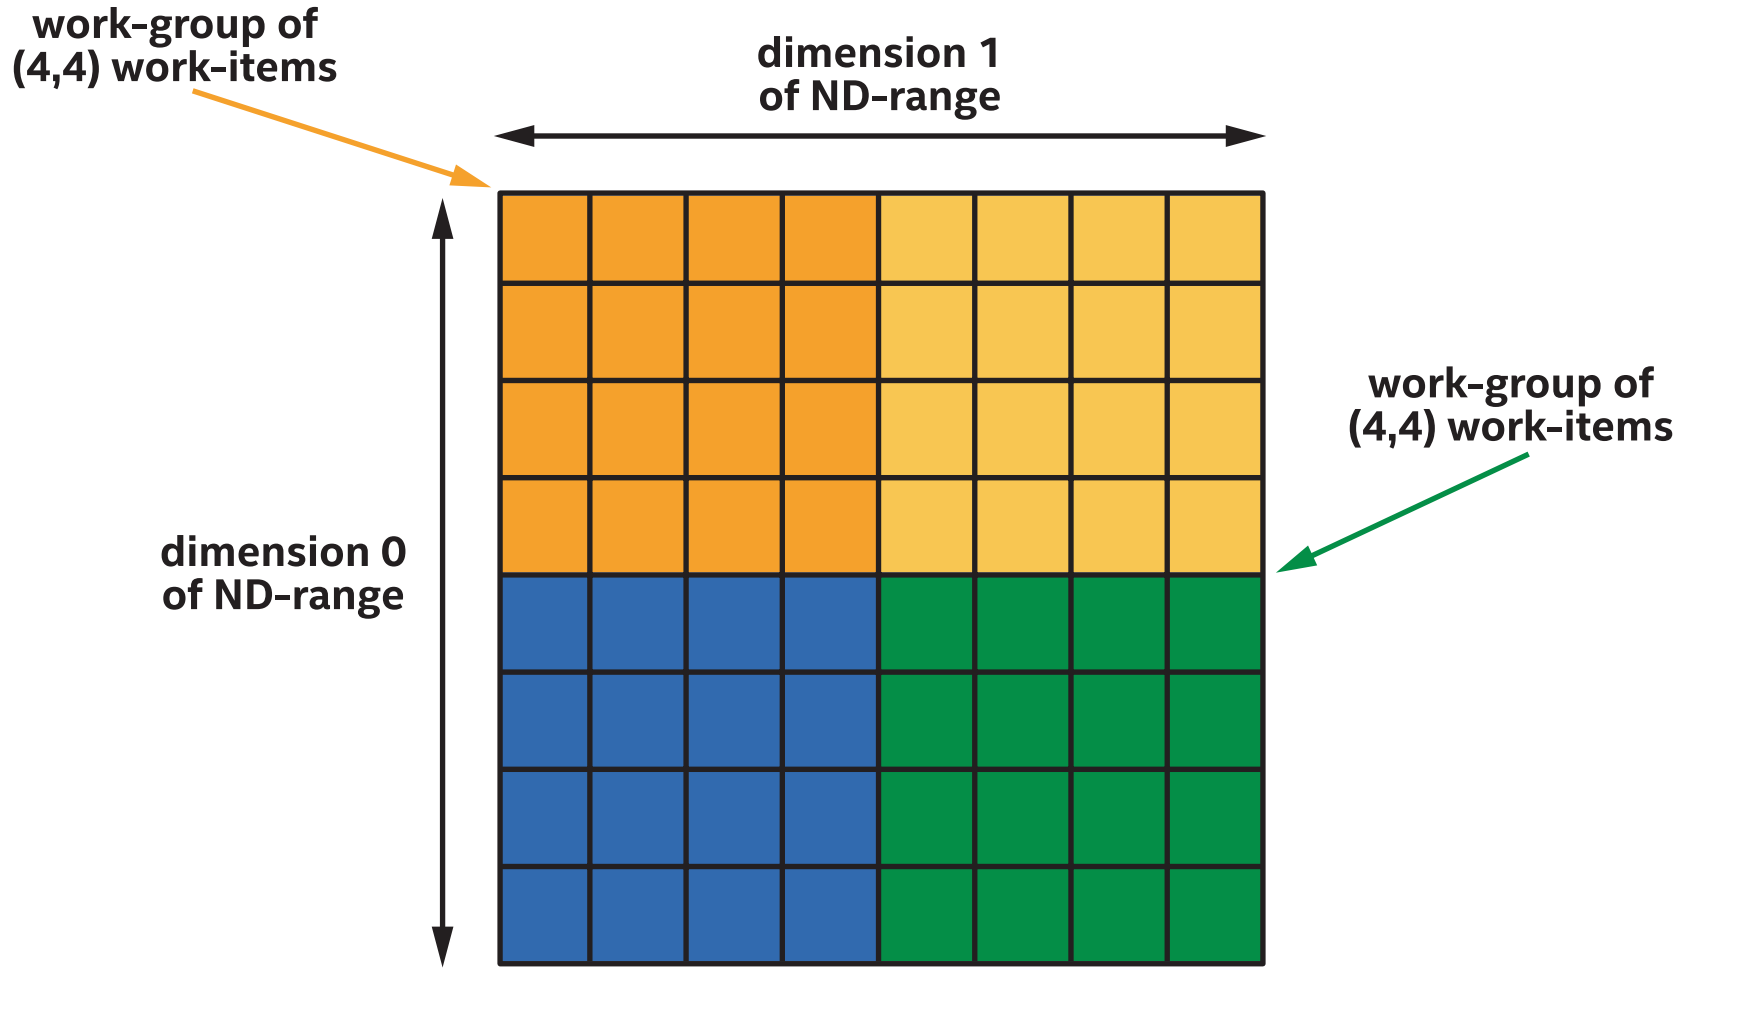
\includegraphics[width=1.\textwidth]{content/chapter-9/images/2}
\end{center}

Figure 9-1 shows an ND-range divided into work-groups, where each work-group is represented by a different color. The work-items in each work-group are guaranteed to execute concurrently, so a work-item may communicate with other work-items that share the same color.\par

Because the work-items in different work-groups are not guaranteed to execute concurrently, a work-item with one color cannot reliably communicate with a work-item with a different color, and a kernel may deadlock if one work-item attempts to communicate with another workitem that is not currently executing. Since we want our kernels to complete execution, we must ensure that when one work-item communicates with another work-item, they are in the same work-group.\par















































